\documentclass[letterpaper, 12pt]{article}

\setlength{\topmargin}{0in}
\setlength{\textheight}{9.0in}
\setlength{\textwidth}{6.5in}
\setlength{\columnsep}{0.25in}
\setlength{\headheight}{0in}
\setlength{\headsep}{0in}
\setlength{\oddsidemargin}{0.0in}
\setlength{\evensidemargin}{0.0in}
\setlength{\topskip}{0in}

\usepackage[utf8]{inputenc}
\usepackage{pgfplots}
\usepackage{amsmath}
\usepackage[ruled,vlined,]{algorithm2e}

\title{CSE380 HW04}
\author{Mason Schechter}
\date{October 29 2020}

\begin{document}

\maketitle
\begin{flushleft}
\section{Introduction}

Here, we will be solving the steady-state heat equation:
\begin{equation} \label{eq:1}
    \ -k \nabla ^2 T (x,y) = q(x,y)\
\end{equation}

where \emph{k} is the thermal conductivity, \emph{T} is the material temperature, and \emph{q} is a heat source term. The expanded form of (1) in 1 dimension is:

\begin{equation}
    \ -k \frac{\delta^2 T(x)}{\delta x^2} = q(x) \
\end{equation}

The expanded form of (1) in 2 dimensions is:

\begin{equation}
    \ -k (\frac{\delta^2 T(x)}{\delta x^2}+\frac{\delta^2 T(y)}{\delta y^2}) = q(x,y) \
\end{equation}

To solve the steady-state heat equation in 1 and 2 dimensions, we will first need to approximate the value of the second derivative terms in these equations. To do this, we will use 2nd- and 4th-order central finite-difference approximations. The resulting linear system from these numerical methods will be solved using two iterative solution mechanisms: Jacobi and Gauss-Seidel.

\section{1 Dimension Approximations}

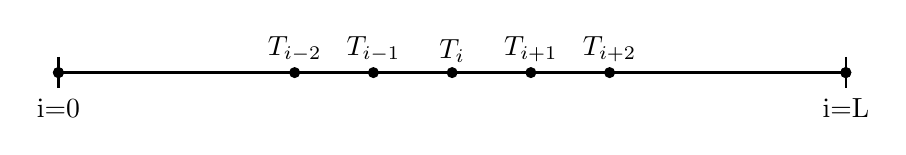
\begin{tikzpicture}[
dot/.style = {circle, fill=black,inner sep=1pt, minimum size=4pt,label={#1},name=#1},
every label/.append style = {inner sep=1pt},thick]
\draw ( 0,0.2) -- + (0,-0.4) node[below] {i=0};
\draw (10,0.2) -- + (0,-0.4) node[below] {i=L};
\draw[thick] (0,0) -- node[below=2mm] {} + (10,0);
    \node[dot] (i=0) at (0,0) {};
    \draw (i=0) node[dot]{};
    \node[dot] (i=L) at (10,0) {};
    \draw (i=L) node[dot]{};
    \node[dot] (T_{i-2}) at (3,0) {};
    \draw (T_{i-2}) node[above]{$T_{i-2}$};
    \node[dot] (T_{i-1}) at (4,0) {};
    \draw (T_{i-1}) node[above]{$T_{i-1}$};
    \node[dot] (T_i) at (5,0) {};
    \draw (T_i) node[above]{$T_i$};
    \node[dot] (T_{i+1}) at (6,0) {};
    \draw (T_{i+1}) node[above]{$T_{i+1}$};
    \node[dot] (T_{i+2}) at (7,0) {};
    \draw (T_{i+2}) node[above]{$T_{i+2}$};

\end{tikzpicture}

Here, we are going to approximate the steady-state heat equation in 1 dimension. In the above diagram, ${T_{i}}$ is the temperature at the point $x=i$, where $x \in [0,L]$. In this node-based scheme, we will be using constant mesh spacing of $N$ points, such that the distance between a point, $T_i$, and the previous point, $T_{i-1}$ or $T(x - \Delta x)$, or the next point, $T_{i+1}$ or $T(x + \Delta x)$, is the same distance $\Delta x$ = $L/N$.
\vskip 15mm
We are assuming:
\begin{enumerate}
    \item The mesh spacing is constant
    \item Dirichlet boundary conditions are applied for any incomplete stencil
    \item The values at the boundaries will be provided through manufactured solutions. 
    \item $T(x)$ is smooth and continuous for all $x \in [0,L]$
    \item The values $T_i$ and $q_i$ are not changing over time
\end{enumerate}


The 2nd-order approximation for the second derivative in (2) is:
\begin{equation}
    \frac{\delta^2 T(x)}{\delta x^2} \approx \frac{T_{i-1} - 2T_i + T_{i+1}}{\Delta x^2}
\end{equation}

Substituting this approximation into (2) gives us:
\begin{equation}
    T_{i-1} - 2T_i + T_{i+1} \approx - \frac{q_i \Delta x^2}{k}
\end{equation}

where the truncation error of this approximation is on the order of $\Delta x^2$. The resulting linear system looks like this:
\[
\begin{bmatrix}
    1 & 0 & 0 & \hdots & \hdots & \hdots & 0\\
    1 & -2 & 1 & 0 & \hdots & \hdots & 0\\
    0 & 1 & -2 & 1 & 0 & \hdots & 0\\
    0 & \ddots & \ddots & \ddots & \ddots & \ddots &  0\\
    0 & \ddots & \ddots & \ddots & \ddots & \ddots &  0\\
    0 & \ddots & \ddots & \ddots & 1 & -2 & 1 \\
    0 & 0 & 0 & 0 & 0 & 0 & 1
    
\end{bmatrix}
\begin{bmatrix}
    T_0 \\
    T_1 \\
    T_2 \\
    \vdots \\
    \vdots \\
    T_{L-1} \\
    T_L
\end{bmatrix}
=
\begin{bmatrix}
    - \frac{q_0 \Delta x^2}{k} \\
    - \frac{q_1 \Delta x^2}{k} \\
    - \frac{q_1 \Delta x^2}{k} \\
    \vdots \\
    - \frac{q_{L-1} \Delta x^2}{k} \\
    - \frac{q_L \Delta x^2}{k}
\end{bmatrix}
\]
Each interior (non-boundary) row contains 3 non-zero entries and $N-3$ zeros.
\vskip 5mm
The 4th-order approximation for the second derivative in (2) is:
\begin{equation}
    \frac{\delta^2 T(x)}{\delta x^2} \approx \frac{-T_{i-2} + 16T_{i-1} - 30T_i + 16T_{i+1} -T_{i+2}}{12 \Delta x^2}
\end{equation}

Substituting this approximation into (2) gives us:
\begin{equation}
    -\frac{1}{12}T_{i-2} + \frac{4}{3}T_{i-1} - \frac{5}{2}T_i + \frac{4}{3}T_{i+1} -\frac{1}{12}T_{i+2} \approx - \frac{q_i \Delta x^2}{k}
\end{equation}
where the truncation error of this approximation is on the order of $\Delta x^4$. The resulting linear system looks like this:
\[
\begin{bmatrix}
    1 & 0 & 0 & \hdots & \hdots & \hdots & \hdots & \hdots & 0\\
    0 & 1 & 0 & 0 & \hdots & \hdots & \hdots & \hdots & 0\\
    -\frac{1}{12} & \frac{4}{3} & -\frac{5}{2} & \frac{4}{3} & -\frac{1}{12} & 0 & \hdots &  \hdots & 0\\
    0 & -\frac{1}{12} & \frac{4}{3} & -\frac{5}{2} & \frac{4}{3} & -\frac{1}{12} & 0 & \hdots &  0\\
    0 & \ddots & \ddots & \ddots & \ddots & \ddots & \ddots & \ddots & 0 \\
    0 & \ddots & \ddots & \ddots & \ddots & \ddots & \ddots & \ddots & 0 \\
    0 & \hdots &  \hdots & 0 & -\frac{1}{12} & \frac{4}{3} & -\frac{5}{2} & \frac{4}{3} & -\frac{1}{12}\\
    0 & 0 & 0 & 0 & 0 & 0 & 0 & 1 & 0 \\
    0 & 0 & 0 & 0 & 0 & 0 & 0 & 0 & 1
    
\end{bmatrix}
\begin{bmatrix}
    T_0 \\
    T_1 \\
    T_2 \\
    \vdots \\
    \vdots \\
    \vdots \\
    T_{L-2} \\
    T_{L-1} \\
    T_L
\end{bmatrix}
=
\begin{bmatrix}
    - \frac{q_0 \Delta x^2}{k} \\
    - \frac{q_1 \Delta x^2}{k} \\
    - \frac{q_2 \Delta x^2}{k} \\
    \vdots \\
    \vdots \\
    \vdots \\
    - \frac{q_{L-2} \Delta x^2}{k} \\
    - \frac{q_{L-1} \Delta x^2}{k} \\
    - \frac{q_L \Delta x^2}{k}
\end{bmatrix}
\]
Each interior row has 5 non-zero entries and $N-5$ zeros.

\section{2 Dimension Approximations}
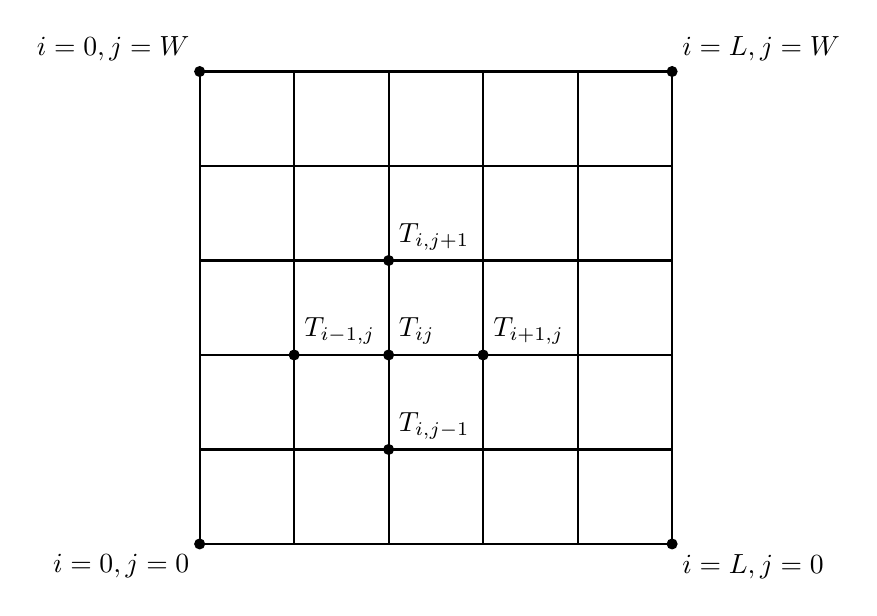
\begin{tikzpicture}[
dot/.style = {circle, fill=black,inner sep=1pt, minimum size=4pt,label={#1},name=#1},
every label/.append style = {inner sep=1pt},
    thick      
                        ]
\draw[step=1.2cm,black,thick]
(0,0) grid (6,6);
    \node[dot] (A) at (0,0) {};
    \draw (A) node[below left]{$i=0, j=0$};
    \node[dot] (B) at (6,0) {};
    \draw (B) node[below right]{$i=L, j=0$};
    \node[dot] (C) at (0,6) {};
    \draw (C) node[above left]{$i=0, j=W$};
    \node[dot] (D) at (6,6) {};
    \draw (D) node[above right]{$i=L, j=W$};
    
    \node[dot] (E) at (2.4,2.4) {};
    \draw (E) node[above right]{$T_{ij}$};
    \node[dot] (F) at (1.2,2.4) {};
    \draw (F) node[above right]{$T_{i-1,j}$};
    \node[dot] (G) at (3.6,2.4) {};
    \draw (G) node[above right]{$T_{i+1,j}$};
    \node[dot] (H) at (2.4,1.2) {};
    \draw (H) node[above right]{$T_{i,j-1}$};
    \node[dot] (I) at (2.4,3.6) {};
    \draw (I) node[above right]{$T_{i,j+1}$};

\end{tikzpicture}

Here, we are going to approximate the steady-state heat equation in 2 dimensions. In the above diagram of our node-based scheme, $T_{ij}$ is the temperature at the point $x=i, y=j$ or $T(x=i, y=j)$, where $ x \in [0,L] $ and $y \in [0, W] $. We are assuming a square domain, such that $L = W$. We will be using the same number of discretization points, $N$, for each dimension, such that $\Delta x = \Delta y = \Delta n$. However, we will need to make a mapping from this 2-D coordinate system to a 1-D vectored system. We will use the equation $h = i + j(N_x) = i + j(N_y)$ where $N_x$ and $N_y$ are the number of discretization points in the x- and y-directions, respectively. Again, they are the same value for the following solutions. Our new mesh grid will look like this:

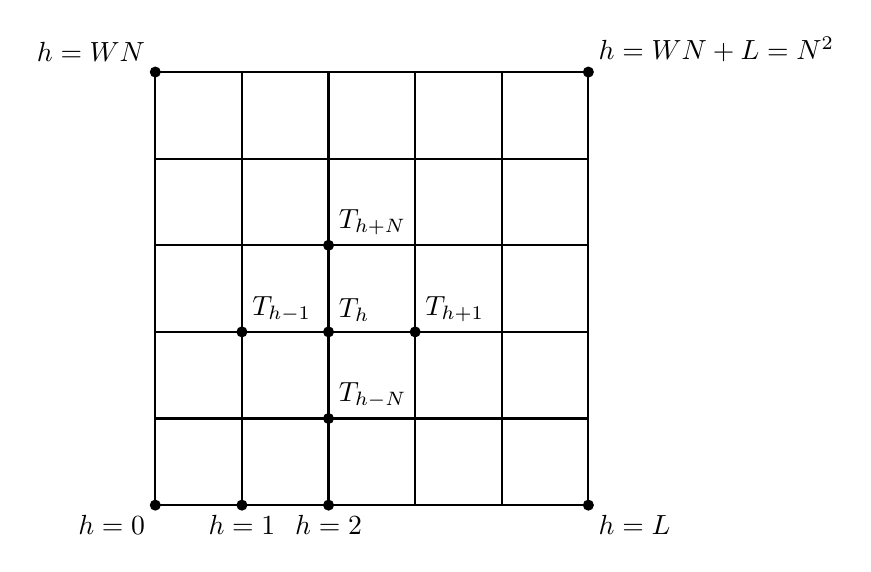
\begin{tikzpicture}[
dot/.style = {circle, fill=black,inner sep=1pt, minimum size=4pt,label={#1},name=#1},
every label/.append style = {inner sep=1pt},thick]
\draw[step=1.1cm,black,thick]
(0,0) grid (5.5,5.5);
    \node[dot] (A) at (0,0) {};
    \draw (A) node[below left]{$h=0$};
    \node[dot] (B) at (5.5,0) {};
    \draw (B) node[below right]{$h = L$};
    \node[dot] (C) at (0,5.5) {};
    \draw (C) node[above left]{$h = WN$};
    \node[dot] (D) at (5.5,5.5) {};
    \draw (D) node[above right]{$h = WN + L = N ^2$};
    \node[dot] (J) at (1.1,0) {};
    \draw (J) node[below]{$h=1$};
    \node[dot] (K) at (2.2,0) {};
    \draw (K) node[below]{$h = 2$};
    
    \node[dot] (E) at (2.2,2.2) {};
    \draw (E) node[above right]{$T_{h}$};
    \node[dot] (F) at (1.1,2.2) {};
    \draw (F) node[above right]{$T_{h-1}$};
    \node[dot] (G) at (3.3,2.2) {};
    \draw (G) node[above right]{$T_{h+1}$};
    \node[dot] (H) at (2.2,1.1) {};
    \draw (H) node[above right]{$T_{h-N}$};
    \node[dot] (I) at (2.2,3.3) {};
    \draw (I) node[above right]{$T_{h+N}$};

\end{tikzpicture}
\vskip 5mm
We are assuming:
\begin{enumerate}
    \item The mesh spacing is constant, such that $N_x$ = $N_y$, therefore $\Delta x$ = $\Delta y$ = $\Delta n$
    \item The domain is square, such that $L=W$
    \item Dirichlet boundary conditions are applied for any incomplete stencil
    \item The values at the boundaries will be provided through manufactured solutions. 
    \item $T(x,y)$ is smooth and continuous for all $x \in [0,L]$ and all $y \in [0,W]$
    \item The values $T_{ij}$ and $q_{ij}$ are not changing over time
\end{enumerate}
\vskip 5mm
The 2nd-order approximation for the second derivative terms in (3) is:
\begin{equation}
    \frac{\delta^2 T(x)}{\delta x^2} \approx \frac{T_{h-1} - 2T_h + T_{h+1}}{\Delta x^2}
\end{equation}

\begin{equation}
    \frac{\delta^2 T(y)}{\delta y^2} \approx \frac{T_{h-N} - 2T_h + T_{h+N}}{\Delta y^2}
\end{equation}


Substituting this approximation into (3) gives us:
\begin{equation}
    T_{h-N} + T_{h-1} - 4T_h + T_{h+1} + T_{h+N} \approx - \frac{q_h \Delta n^2}{k}
\end{equation}
where the truncation error of this approximation is on the order of $\Delta n^2$. The resulting linear system looks like this:
\[
\begin{bmatrix}

    \vdots & \ddots & \ddots & \ddots & \ddots & \ddots & \ddots & \ddots & \ddots & \vdots \\
    \hdots & N zeros & 1 & -4 & 1 & N zeros & 1 & 0 & \hdots & \hdots\\
    \hdots & 1 & N zeros & 1 & -4 & 1 & N zeros & 1 & 0 & \hdots \\
    \hdots & 0 & 1 & N zeros & 1 & -4 & 1 & N zeros & 1 &  0\\
    \hdots & 0 & \ddots & \ddots & \ddots & \ddots & \ddots & \ddots & \ddots & 0 \\
    \hdots & 0 & \ddots & \ddots & \ddots & \ddots & \ddots & \ddots & \ddots & 0 \\
    \hdots & 0 & \hdots &  \hdots & \hdots & \hdots & 0 & 1 & 0 & 0\\
    \hdots & 0 & 0 & 0 & 0 & 0 & 0 & 0 & 1 & 0 \\
    \hdots & 0 & 0 & 0 & 0 & 0 & 0 & 0 & 0 & 1
    
\end{bmatrix}
\begin{bmatrix}
    \vdots \\
    T_{h-1} \\
    T_{h} \\
    T_{h+1} \\
    \vdots \\
    \vdots \\
    \vdots \\
    T_{N^2-2} \\
    T_{N^2-1} \\
    T_{N^2}
\end{bmatrix}
=
\begin{bmatrix}
    - \frac{q_0 \Delta n^2}{k} \\
    - \frac{q_1 \Delta n^2}{k} \\
    - \frac{q_2 \Delta n^2}{k} \\
    \vdots \\
    \vdots \\
    \vdots \\
    - \frac{q_{N^2-2} \Delta n^2}{k} \\
    - \frac{q_{N^2-1} \Delta n^2}{k} \\
    - \frac{q_{N^2} \Delta n^2}{k}
\end{bmatrix}
\]
Each interior row contains 5 non-zero entries and N-5 zeros.
\vskip 5mm
The 4th-order approximation for the second derivative terms in (3) is:
\begin{equation}
    \frac{\delta^2 T(x)}{\delta x^2} \approx \frac{-T_{h-2} + 16T_{h-1} - 30T_h + 16T_{h+1} -T_{h+2}}{12 \Delta n^2}
\end{equation}

\begin{equation}
    \frac{\delta^2 T(y)}{\delta y^2} \approx \frac{-T_{h-2N} + 16T_{h-N} - 30T_h + 16T_{h+N} -T_{h+2N}}{12 \Delta n^2}
\end{equation}
Substituting this approximation into (3) gives us:
\begin{equation}
    -\frac{1}{12}T_{h-2N} + \frac{4}{3}T_{h-N} - \frac{1}{12}T_{h-2} + \frac{4}{3}T_{h-1} + 5T_h + \frac{4}{3}T_{h+1} - \frac{1}{12}T_{h+2} + \frac{4}{3}T_{h+N} - \frac{1}{12}T_{h+2N} \approx -\frac{q_h\Delta n^2}{12k}
\end{equation}
where the truncation error of this approximation is on the order of $\Delta n^4$. The resulting coefficient matrix looks like this:
\[ A =
\begin{bmatrix}

    \vdots & \ddots & \ddots & \ddots & \ddots & \ddots & \ddots & \ddots & \ddots & \vdots \\
    \hdots & N zeros & - \frac{1}{12} & \frac{4}{3} & 5 & \frac{4}{3} & - \frac{1}{12} & N zeros & \frac{4}{3} & N zeros\\
    \hdots & \frac{4}{3} & N zeros & - \frac{1}{12} & \frac{4}{3} & 5 & \frac{4}{3} & - \frac{1}{12} & N zeros & \hdots \\
    \hdots & N zeros & \frac{4}{3} & N zeros & - \frac{1}{12} & \frac{4}{3} & 5 & \frac{4}{3} & - \frac{1}{12} & N zeros\\
    \hdots & - \frac{1}{12} & N zeros & \frac{4}{3} & N zeros & - \frac{1}{12} & \frac{4}{3} & 5 & \frac{4}{3} & - \frac{1}{12} \\
    \hdots & 0 & - \frac{1}{12} & N zeros & \frac{4}{3} & N zeros & - \frac{1}{12} & \frac{4}{3} & 5 & \frac{4}{3} \\
    \hdots & 0 & \ddots &  \ddots & \ddots & \ddots & \ddots & \ddots & \ddots & \ddots\\
    \hdots & 0 & 0 & 0 & 0 & 0 & 0 & 0 & 1 & 0 \\
    \hdots & 0 & 0 & 0 & 0 & 0 & 0 & 0 & 0 & 1
\end{bmatrix}
\]
Each interior row has 9 non-zero entries. The resulting linear system looks like this:
\[ A
\begin{bmatrix}
    \vdots \\
    T_{h-1} \\
    T_{h} \\
    T_{h+1} \\
    \vdots \\
    \vdots \\
    \vdots \\
   \vdots \\
    T_{N^2-1} \\
    T_{N^2}
\end{bmatrix}
=
\begin{bmatrix}
    - \frac{q_0 \Delta n^2}{k} \\
    - \frac{q_1 \Delta n^2}{k} \\
    - \frac{q_2 \Delta n^2}{k} \\
    \vdots \\
    \vdots \\
    \vdots \\
    - \frac{q_{N^2-2} \Delta n^2}{k} \\
    - \frac{q_{N^2-1} \Delta n^2}{k} \\
    - \frac{q_{N^2} \Delta n^2}{k}
\end{bmatrix}
\]

\section{Jacobi Method}
\begin{algorithm}
\SetAlgoLined
 Initialize two, 1x$N^2$ T vectors, $T_{old}$ and $T_{new}$\;
 Set each value in $T_{old}$ to 0\;
 \While{currentError $>$ errorThreshold}{
  \For{each h from 0 to $N^2$}{
   solve for $T_h$ with the values from $T_{old}$ for the other components\;
   
   store result $T_h$ in $T_{new}$\;
  }
  currentError = \|$T_{old}$ $-$ $T_{new}$\| $ / $ $T_{old}$ \;
  $T_{old}$ $=$ $T_{new}$
  }
\end{algorithm}

Estimated memory needed \approx  $8 bytes x 2N^2$

\section{Gauss-Seidel Method}
\begin{algorithm}
\SetAlgoLined
 Initialize two, $1xN^2$ T vectors, $T_{old}$ and $T_{new}$\;
 Set each value in $T_{old}$ to 0\;
 $T_{new}$ = $T_{old}$ \;
 \While{currentError $>$ errorThreshold}{
  \For{each h from 0 to N^2}{
   solve for $T_h$ with the values from $T_{new}$ for the other components\;
   
   store result $T_h$ in $T_{new}$\;
  }
  currentError = \|$T_{old}$ $-$ $T_{new}$\| $ / $ $T_{old}$ \;
  $T_{old}$ = $T_{new}$ \;
  }
\end{algorithm}

Estimated memory needed \approx  $8 bytes x 2N^2$




\end{flushleft}

\end{document}
